\chapter{От частиц к простому квантовому полю}

Построим простое квантовое поле еще раз, но под несколько иным углом зрения. К квантовой теории поля ведут два пути. Можно начать с частиц и понять, почему поле является для них естественным языком, или начать с волнового поля и понять, почему его возбуждения квантуются. Оба пути полезны. Здесь мы придерживаемся первого.

Обычная квантовая механика может описывать одну частицу, две частицы или любое другое фиксированное число. Природа не соблюдает этого ограничения. Число фотонов в комнате меняется всякий раз, когда источники света испускают или поглощают излучение. Нестабильные частицы распадаются. При бета-распаде, например,
\begin{equation}
n\longrightarrow p+e^-+\bar{\nu}_e,
\end{equation}
так что одновременно меняются численности нескольких видов частиц. Поэтому нам нужна одна квантовая механика, достаточно большая, чтобы охватывать любое возможное число заполнения и, в конечном счете, процессы перехода между ними.

Пока что мы сильно упростим задачу. Есть один вид нерелятивистской частицы. Сначала мы расширим пространство ее состояний так, чтобы в нем могло содержаться любое число частиц, и лишь затем обсудим большее число видов, релятивистский случай, рассеяние и распад. Никакая часть математики здесь не является особенно трудной, но смена точки зрения абстрактна. Стоит продвигаться достаточно медленно, чтобы обозначения не скрыли саму идею.

\section{Одночастичная отправная точка}

Начнем с одной частицы в состоянии \(|\psi\rangle\). Ее волновая функция в координатном представлении имеет вид
\begin{equation}
\psi(x)=\langle x|\psi\rangle.
\label{eq:l07-wavefunction}
\end{equation}
Эта строчная \(\psi\) есть обычная комплекснозначная функция. Это еще не квантовое поле и не оператор в пространстве состояний многих частиц.

Согласно правилу Борна,
\begin{equation}
\rho_\psi(x)=|\psi(x)|^2=\psi^*(x)\psi(x)
\label{eq:l07-born-density}
\end{equation}
есть плотность вероятности обнаружить частицу в точке \(x\). Для нормированного состояния
\begin{equation}
\int dx\,\psi^*(x)\psi(x)=1.
\label{eq:l07-one-particle-normalization}
\end{equation}
Правая часть есть полная вероятность. Поскольку в этой задаче имеется ровно одна частица, она по совпадению также равна числу частиц. Это совпадение станет полезной подсказкой, хотя здесь оно тривиально.

\begin{classroomqa}
\lecturetimestamp{00:09:13}
\audiencequestion{Почему плотность вероятности должна иметь вид \(\psi^*(x)\psi(x)\)?}
\lecturerresponse{Это правило Борна, один из постулатов квантовой механики. Амплитуда для результата измерения положения \(x\) равна \(\langle x|\psi\rangle\); плотность вероятности равна квадрату ее модуля. Она не выводится из используемого позднее построения поля.}
\end{classroomqa}

\section{Моды, ортогональность и полнота}

В одночастичном гильбертовом пространстве есть много полезных базисов. Один базис образуют собственные состояния положения. Другой образуют собственные состояния любого эрмитова оператора с обычными оговорками относительно вырождений и непрерывных спектров. Поскольку энергия вскоре станет важной, выберем полный ортонормированный набор одночастичных собственных состояний энергии
\begin{equation}
|1\rangle,\ |2\rangle,\ldots,
\qquad
\psi_i(x)=\langle x|i\rangle.
\end{equation}

Частица в ящике делает индекс \(i\) наглядным. Волновая функция основного состояния не имеет внутренних узлов, у следующего состояния один узел, а у более высоких состояний осцилляции происходят быстрее. Для идеальной бесконечно глубокой прямоугольной ямы это, по существу, синусоиды.

\begin{figure}[htbp]
\centering
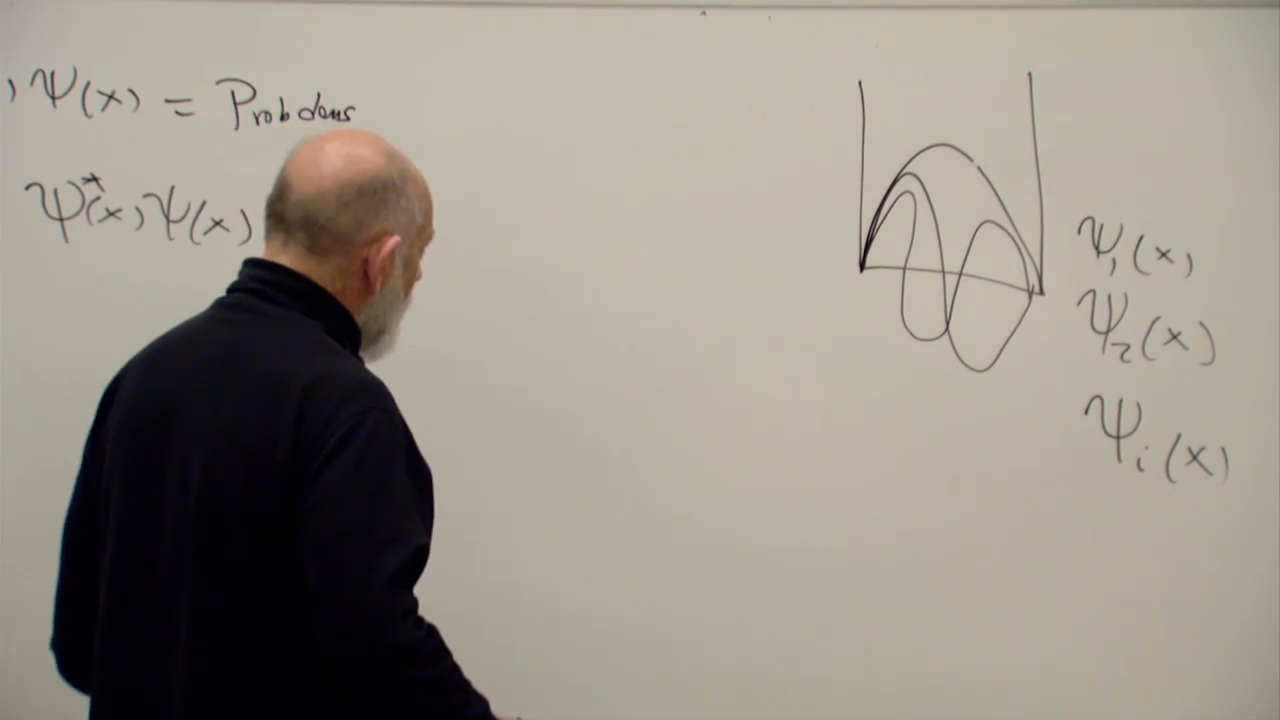
\includegraphics[width=0.94\linewidth]{lecture_07_frame_01.png}
\caption{Моды в ящике на лекционной доске. Следы слева — это одночастичная плотность Борна и нормировка; яма справа показывает \(\psi_1(x)\), \(\psi_2(x)\) и общее обозначение \(\psi_i(x)\).}
\lectureframe{00:08:25}
\end{figure}

Ту же структуру мод можно отделить от перекрытия на кадре с доски:
\begin{figure}[htbp]
\centering
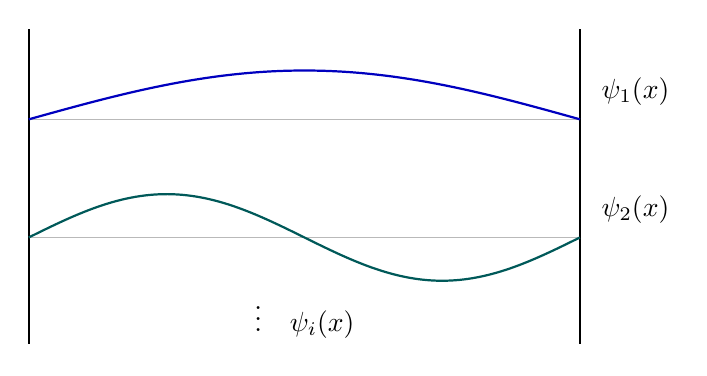
\begin{tikzpicture}[x=1cm,y=1cm]
  \draw[thick] (0,0) -- (0,4.0);
  \draw[thick] (7,0) -- (7,4.0);
  \draw[gray!55] (0,2.85) -- (7,2.85);
  \draw[gray!55] (0,1.35) -- (7,1.35);
  \draw[blue!75!black,thick,domain=0:7,samples=120]
    plot (\x,{2.85+0.62*sin(180*\x/7)});
  \draw[teal!70!black,thick,domain=0:7,samples=120]
    plot (\x,{1.35+0.55*sin(360*\x/7)});
  \node[right] at (7.15,3.20) {$\psi_1(x)$};
  \node[right] at (7.15,1.70) {$\psi_2(x)$};
  \node at (3.5,0.38) {$\vdots\quad\psi_i(x)$};
\end{tikzpicture}
\caption{Чистая реконструкция качественного эскиза ящика. Вертикальные смещения лишь разделяют две волновые функции для наглядности.}
\end{figure}

Ортонормированность выражается равенством
\begin{equation}
\int dx\,\psi_i^*(x)\psi_j(x)=\delta_{ij}.
\label{eq:l07-orthonormality}
\end{equation}
Если \(i=j\), состояние нормировано и интеграл равен единице. Если \(i\ne j\), два состояния ортогональны и интеграл обращается в нуль.

Полнота — столь же важное утверждение
\begin{equation}
\sum_i |i\rangle\langle i|=\mathbf 1.
\label{eq:l07-resolution}
\end{equation}
Каждый оператор \(|i\rangle\langle i|\) проектирует на одно направление базиса; сумма по полному базису дает единичный оператор. Действуя на произвольный вектор, она просто разлагает этот вектор на компоненты и снова собирает его.

Теперь вставим равенство~\eqref{eq:l07-resolution} между двумя состояниями положения:
\begin{align}
\langle y|x\rangle
&=\sum_i\langle y|i\rangle\langle i|x\rangle \\
&=\sum_i\psi_i(y)\psi_i^*(x) \\
&=\delta(y-x).
\label{eq:l07-position-completeness}
\end{align}
Звездочка должна стоять у того множителя, чей порядок бра и кет равен \(\langle i|x\rangle\). Перестановка \(x\) и \(y\) дает комплексно-сопряженную, но эквивалентную форму. Таким образом, всякий полный ортонормированный базис задает представление дельта-функции. Синусы, косинусы, волновые функции осциллятора и собственные функции энергии выполняют одну и ту же роль.

\begin{classroomqa}
\lecturetimestamp{00:13:43}
\audiencequestion{Должна ли вторая волновая функция в сумме полноты стоять с комплексным сопряжением?}
\lecturerresponse{Да. При порядке \(\langle y|i\rangle\langle i|x\rangle\) множители равны \(\psi_i(y)\psi_i^*(x)\). Если держать порядок бра и кет на виду, звездочку не придется угадывать или ставить не туда.}
\end{classroomqa}

Это вся одночастичная математика, которая нам понадобится. Теперь мы меняем пространство состояний.

\section{Пространство Фока как более широкое пространство состояний}

Для многих тождественных частиц удобный базис фиксирует, сколько частиц занимает каждую одночастичную моду:
\begin{equation}
|n_1,n_2,n_3,\ldots\rangle.
\label{eq:l07-fock-basis}
\end{equation}
Целое число \(n_i\) есть число заполнения моды \(i\). Этот кет — не одночастичное состояние, записанное в необычной нотации. Он принадлежит большему гильбертову пространству, содержащему сектор с нулем частиц, все одночастичные состояния, все двухчастичные состояния и так далее. Это большее пространство называется пространством Фока.

Чтобы изменять заполнения, введем для каждой моды оператор рождения и оператор уничтожения,
\begin{equation}
a_i^\dagger,\qquad a_i.
\end{equation}
Первый добавляет одну частицу в моду \(i\), а второй убирает одну. На этом этапе язык гармонического осциллятора служит средством учета: здесь не обязательно буквально колеблется пружина. Алгебра осциллятора дает нам в точности тот аппарат, который нужен для повышения и понижения чисел заполнения.

Оператор числа заполнения моды имеет вид
\begin{equation}
\begin{aligned}
N_i&=a_i^\dagger a_i,\\
N_i|n_1,\ldots,n_i,\ldots\rangle
&=n_i|n_1,\ldots,n_i,\ldots\rangle.
\end{aligned}
\end{equation}
Вакуум есть
\begin{equation}
|0\rangle\equiv|0,0,0,\ldots\rangle,
\qquad
a_i|0\rangle=0
\quad\text{for every }i.
\label{eq:l07-vacuum}
\end{equation}
Поэтому одночастичное состояние в моде \(i\) равно
\begin{equation}
|i\rangle=a_i^\dagger|0\rangle.
\label{eq:l07-mode-created}
\end{equation}
Один и тот же символ \(|i\rangle\) теперь можно понимать либо как базисный вектор одночастичного пространства, либо как тот же вектор, вложенный в одночастичный сектор пространства Фока. Это вложение задается уравнением~\eqref{eq:l07-mode-created}; из окружающего контекста ясно, о каком пространстве идет речь.

\section{Объединение мод в поле}

Определим поля уничтожения и рождения как
\begin{equation}
\Psi(x)=\sum_i \psi_i(x)a_i,
\qquad
\Psi^\dagger(x)=\sum_i \psi_i^*(x)a_i^\dagger.
\label{eq:l07-field-expansion}
\end{equation}
Заглавная буква здесь существенна. Функции со строчной буквой \(\psi_i(x)\) — это комплексные числа; заглавная \(\Psi(x)\) есть оператор в пространстве Фока. В каждой пространственной точке \(x\) уравнение~\eqref{eq:l07-field-expansion} задает другую линейную комбинацию операторов мод. Именно это и означает операторнозначная функция положения.

Для свободных частиц функциями мод могут служить плоские волны \(e^{ikx}\). Тогда уравнение~\eqref{eq:l07-field-expansion} представляет собой разложение Фурье, за исключением того, что его коэффициенты Фурье — операторы, а не числа. В старой терминологии обычные комплексные числа называются \(c\)-числами, а квантовые операторы — \(q\)-числами. Функции мод являются \(c\)-числами и коммутируют со всем; операторный характер несут \(a_i\) и \(a_i^\dagger\).

Ни \(\Psi\), ни \(\Psi^\dagger\) не являются эрмитовыми. Они взаимно сопряжены. Две комбинации
\begin{equation}
\Psi+\Psi^\dagger,
\qquad
i(\Psi^\dagger-\Psi)
\label{eq:l07-hermitian-combinations}
\end{equation}
эрмитовы и могут представлять наблюдаемые. Однако пока поля наиболее полезны как средства, которые локально рождают, уничтожают и считают частицы.

\begin{classroomqa}
\lecturetimestamp{00:21:05}
\audiencequestion{Что означает, что оператор зависит от \(x\)?}
\lecturerresponse{Это означает, что каждому значению \(x\) соответствует свой оператор. Пространственная зависимость содержится в обычных функциях мод, тогда как каждая получающаяся линейная комбинация действует в одном и том же пространстве Фока.}
\end{classroomqa}

\section{Что делает поле рождения}

Определение становится полезным, когда мы спрашиваем, что оно делает. Начнем с собственного состояния положения в одночастичном секторе и вставим разложение единицы:
\begin{align}
|x\rangle
&=\sum_i |i\rangle\langle i|x\rangle \\
&=\sum_i a_i^\dagger|0\rangle\,\psi_i^*(x) \\
&=\Psi^\dagger(x)|0\rangle.
\label{eq:l07-local-creation}
\end{align}
Таким образом, \(a_i^\dagger\) рождает частицу в определенной моде \(i\), тогда как \(\Psi^\dagger(x)\) рождает частицу, локализованную в точке \(x\). В идеализированном базисе положений такая локализация понимается в смысле распределений; при физическом приготовлении использовался бы узкий волновой пакет, но алгебраический смысл остается тем же.

\begin{classroomqa}
\lecturetimestamp{00:24:48}
\audiencequestion{Является ли \(\sum_i|i\rangle\langle i|\) проектором?}
\lecturerresponse{Каждое слагаемое есть проектор на одно базисное состояние. Полная сумма есть сама единица и называется разложением единицы. Ее вставка не меняет никакого состояния, но выявляет компоненты состояния в выбранном базисе.}
\end{classroomqa}

Уравнение~\eqref{eq:l07-local-creation} дает первое прямое истолкование поля в терминах частиц. Мы не просто прикрепили пространственную метку к абстрактному оператору. Мы построили операцию, создающую частицу в этой пространственной точке.

\begin{classroomqa}
\lecturetimestamp{00:28:20}
\audiencequestion{Следует ли помечать поле рождения в координатном представлении звездочкой или даггером?}
\lecturerresponse{Для сопряжения оператора используйте даггер. Звездочки обозначают комплексное сопряжение обычных волновых функций \(\psi_i(x)\); даггер должен стоять у \(a_i^\dagger\) и \(\Psi^\dagger(x)\).}
\end{classroomqa}

\begin{classroomqa}
\lecturetimestamp{00:28:36}
\audiencequestion{Можно ли в разложении по модам переставлять операторы рождения через волновые функции?}
\lecturerresponse{Да. \(\psi_i(x)\) — \(c\)-числа, поэтому они коммутируют с любым оператором. Осторожность нужна только при изменении порядка некоммутирующих операторов, таких как \(a_i\) и \(a_j^\dagger\).}
\end{classroomqa}

\section{От плотности вероятности к плотности частиц}

Теперь немного поиграем с полем. Первое естественное выражение таково:
\begin{equation}
\int dx\,\Psi^\dagger(x)\Psi(x).
\end{equation}
Оно похоже на одночастичный нормировочный интеграл, но теперь его множители — операторы. Подставим разложения по модам, не меняя их порядка:
\begin{align}
\int dx\,\Psi^\dagger(x)\Psi(x)
&=\int dx
\left(\sum_i a_i^\dagger\psi_i^*(x)\right)\\
&\qquad\times\left(\sum_j a_j\psi_j(x)\right) \\
&=\sum_{i,j}a_i^\dagger a_j
\int dx\,\psi_i^*(x)\psi_j(x) \\
&=\sum_{i,j}a_i^\dagger a_j\,\delta_{ij} \\
&=\sum_i a_i^\dagger a_i.
\label{eq:l07-number-derivation}
\end{align}
Следовательно, оператор полного числа частиц равен
\begin{equation}
N=\sum_i N_i
=\int dx\,\Psi^\dagger(x)\Psi(x).
\label{eq:l07-total-number}
\end{equation}
Для обсуждаемых состояний возбуждения с конечной энергией числа заполнения убывают при достаточно большой энергии моды, так что эта сумма обычно конечна, хотя список возможных мод бесконечен.

Подынтегральное выражение — это оператор локальной плотности частиц:
\begin{equation}
n(x)=\Psi^\dagger(x)\Psi(x).
\label{eq:l07-density}
\end{equation}
Строго говоря, плотность в математической точке не измеряют. Для малой области \(R\) измеряют
\begin{equation}
N_R=\int_R dx\,n(x),
\label{eq:l07-regional-number}
\end{equation}
число частиц в этой области. Как и любая квантовая наблюдаемая, \(N_R\) не обязано иметь определённое значение в произвольном состоянии. Повторные приготовления могут давать разные результаты.

\begin{classroomqa}
\lecturetimestamp{00:36:27}
\audiencequestion{Является ли \(\Psi^\dagger(x)\Psi(x)\) многочастичной плотностью вероятности?}
\lecturerresponse{Его прямой смысл — плотность частиц. Многочастичная амплитуда вероятности, вообще говоря, зависит от координат всех частиц. Напротив, локальная билинейная комбинация при интегрировании по этой области подсчитывает число частиц в ней.}
\end{classroomqa}

\begin{classroomqa}
\lecturetimestamp{00:38:28}
\audiencequestion{Действуют ли операторы \(a_i\) и \(a_i^\dagger\) только на векторы состояния, а не на одночастичные волновые функции?}
\lecturerresponse{Да. Они действуют на состояния пространства Фока, такие как \(|n_1,n_2,\ldots\rangle\). Одночастичные модовые функции, которыми они умножаются, — обычные числа и не являются теми объектами, на которые действуют эти лестничные операторы.}
\end{classroomqa}

Кеты чисел заполнения образуют базис, а не наиболее общее состояние. Из них можно строить суперпозиции, в том числе такие, в которых одно и то же полное число по-разному распределено по модам. Для нейтральных частиц, таких как фотоны, можно также суперпонировать разные полные числа частиц. Оператор в уравнении~\eqref{eq:l07-regional-number} сохраняет один и тот же операциональный смысл во всех таких состояниях.

\begin{classroomqa}
\lecturetimestamp{00:40:01}
\audiencequestion{Если разделить плотность частиц на полное число, станет ли она плотностью вероятности обнаружить частицу в \(x\)?}
\lecturerresponse{При фиксированном \(N\) и большом числе частиц \(N_R/N\) является относительной частотой и обычно очень хорошо соответствует одночастичной вероятности. Это не операторное тождество, отождествляющее результат одного измерения с вероятностью. Измеренное число флуктуирует, обычно на величину порядка \(\sqrt N\) в картине независимых частиц, и в отдельной исключительной реализации оно может сильно отличаться от вероятности, хотя такая реализация маловероятна.}
\end{classroomqa}

\begin{classroomqa}
\lecturetimestamp{00:42:25}
\audiencequestion{Что происходит с сохранением заряда в суперпозиции одноэлектронного состояния и состояния без электронов?}
\lecturerresponse{Это не тот вид суперпозиции, который используют для замкнутого сектора с фиксированным электрическим зарядом. Можно суперпонировать разные распределения с одним и тем же полным зарядом. Фотоны не несут электрического заряда, поэтому разные секторы с различным числом фотонов такой проблемы не создают. Числа электронов и позитронов также могут изменяться совместно, тогда как суммарный заряд остаётся фиксированным.}
\end{classroomqa}

\section{Энергия независимых частиц}

Следующая наблюдаемая — энергия. Сначала ограничимся частицами, которые не взаимодействуют друг с другом. В разреженной системе это часто хорошее приближение. Даже фотоны в принципе взаимодействуют через процессы более высокого порядка, но обычное лабораторное излучение достаточно разрежено, так что описание независимыми частицами превосходно.

Пусть \(\omega_i\) обозначает энергию одной частицы в моде \(i\), при \(\hbar=1\). Под модой здесь понимается одно одночастичное состояние. Тогда полный гамильтониан имеет вид
\begin{equation}
H=\sum_i\omega_i N_i
=\sum_i\omega_i a_i^\dagger a_i.
\label{eq:l07-mode-hamiltonian}
\end{equation}
Каждая занятая мода вносит свою одночастичную энергию по одному разу на каждую частицу.

\begin{classroomqa}
\lecturetimestamp{00:48:16}
\audiencequestion{Является ли \(\omega_i\) функцией положения?}
\lecturerresponse{Нет. Это собственное значение энергии, связанное с модой \(i\). Функция \(\psi_i(x)\) зависит от положения; \(\omega_i\) зависит от того, какой энергетический уровень выбран.}
\end{classroomqa}

Значения \(\omega_i\) определяются стационарным одночастичным уравнением Шрёдингера. Определим
\begin{equation}
h=-\frac{\nabla^2}{2m}+V(x).
\label{eq:l07-one-particle-h}
\end{equation}
Тогда
\begin{equation}
h\psi_i(x)=\omega_i\psi_i(x).
\label{eq:l07-schrodinger-eigenvalue}
\end{equation}
В одном измерении оператор импульса равен \(p=-i\partial_x\), и \(p^2/(2m)\) принимает вид \(-\partial_x^2/(2m)\). В трёх измерениях три вторые производные объединяются в \(-\nabla^2/(2m)\).

\begin{figure}[htbp]
\centering
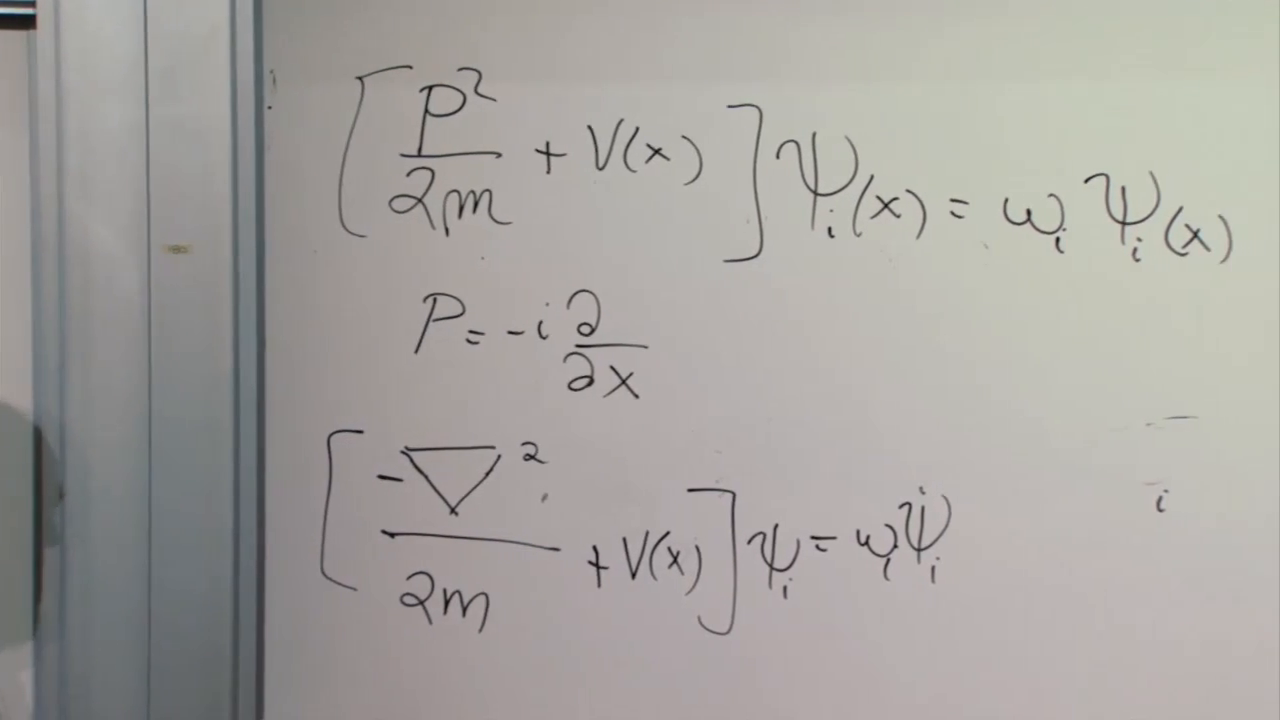
\includegraphics[width=0.94\linewidth]{lecture_07_frame_02.png}
\caption{Переход на доске от \(p^2/(2m)+V(x)\) к дифференциальной форме одночастичного уравнения Шрёдингера на собственные значения. В ~\eqref{eq:l07-schrodinger-eigenvalue} приведена его аккуратно восстановленная запись.}
\lectureframe{00:54:10}
\end{figure}

Для произвольной нормированной одночастичной волновой функции знакомое среднее значение имеет вид
\begin{equation}
\langle h\rangle_\psi
=\int dx\,\psi^*(x)h\psi(x).
\label{eq:l07-one-particle-energy-expectation}
\end{equation}
Многочастичная формула напрашивается, если заменить волновую функцию со строчной буквой операторнозначным полем. Это ещё не доказательство; это догадка, правильность которой мы сейчас проверим:
\begin{equation}
H=\int dx\,\Psi^\dagger(x)h\Psi(x).
\label{eq:l07-field-hamiltonian}
\end{equation}

\section{Сначала ответ, затем доказательство}

Подставим ~\eqref{eq:l07-field-expansion} в предложенный гамильтониан:
\begin{align}
\int dx\,\Psi^\dagger h\Psi
&=\int dx
\left(\sum_i a_i^\dagger\psi_i^*(x)\right)
h\left(\sum_j a_j\psi_j(x)\right) \\
&=\sum_{i,j}a_i^\dagger a_j
\int dx\,\psi_i^*(x)h\psi_j(x).
\label{eq:l07-h-expanded}
\end{align}
Дифференциальный оператор \(h\) действует на зависящую от \(x\) волновую функцию \(\psi_j(x)\), а не на оператор моды \(a_j\). Согласно уравнению Шрёдингера,
\begin{equation}
h\psi_j(x)=\omega_j\psi_j(x).
\end{equation}
Следовательно,
\begin{align}
\int dx\,\Psi^\dagger h\Psi
&=\sum_{i,j}a_i^\dagger a_j\omega_j
\int dx\,\psi_i^*(x)\psi_j(x) \\
&=\sum_{i,j}a_i^\dagger a_j\omega_j\delta_{ij} \\
&=\sum_j\omega_j a_j^\dagger a_j.
\label{eq:l07-h-proof}
\end{align}
Это в точности уравнение~\eqref{eq:l07-mode-hamiltonian}. Локальное полевое выражение и сумма энергий всех частиц — один и тот же оператор.

\begin{figure}[htbp]
\centering
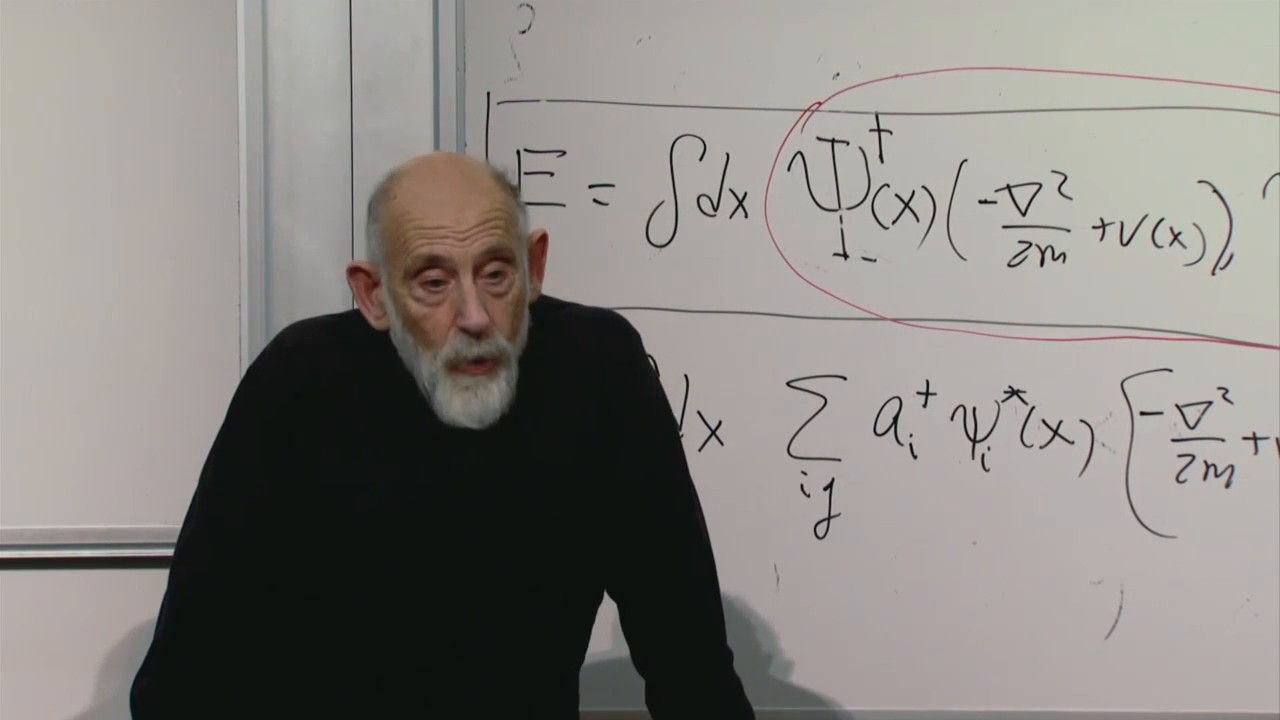
\includegraphics[width=0.94\linewidth]{lecture_07_frame_03.png}
\caption{Полевой гамильтониан, выделенный на доске, а под ним — начало доказательства через разложение по модам. Кадр лекции сохранён как свидетельство; уравнения~\eqref{eq:l07-field-hamiltonian}--\eqref{eq:l07-h-proof} восстанавливают полную алгебру.}
\lectureframe{01:05:34}
\end{figure}

В этом выводе ни один оператор рождения не переставлялся через оператор уничтожения. Порядок \(a_i^\dagger a_j\) сохраняется от начала до конца. Свободно перемещаются только волновые функции, являющиеся \(c\)-числами, и соответствующие им собственные значения.

\section{Почему это поле}

Почему \(\Psi(x)\) называют полем? Потому что это операторнозначная величина, определённая в каждой точке пространства, а эрмитовы комбинации или билинейные выражения, построенные из неё, являются локальными наблюдаемыми. Плотность \(n(x)\) и приведённое ниже локальное выражение для энергии — два примера. За этим словом не скрывается никакого дополнительного математического критерия.

Это поле — не электромагнитное поле. Оно описывает тот нерелятивистский вид частиц, который задаёт одночастичные моды и гамильтониан \(p^2/(2m)+V\): например, медленно движущиеся атомы, нейтроны, протоны или электроны. Эти частицы являются квантами соответствующего поля в том же структурном смысле, в каком фотоны являются квантами электромагнитного поля.

\begin{classroomqa}
\lecturetimestamp{01:02:45}
\audiencequestion{Где при переходе от многочастичной системы к приведённой выше формуле появилось поле?}
\lecturerresponse{Оно появляется в уравнении~\eqref{eq:l07-field-expansion}: \(\Psi(x)\) — оператор в каждой точке пространства. Последующие выводы показывают, что его локальные произведения измеряют плотности частиц и энергии. Зависимость от положения вместе с операторным содержанием и образует именно ту полевую структуру, которая здесь строится.}
\end{classroomqa}

\section{Локальная плотность энергии}

В ~\eqref{eq:l07-field-hamiltonian} полная энергия записывается как интеграл по пространству,
\begin{equation}
\begin{aligned}
H&=\int dx\,\mathcal H(x),\\
\mathcal H(x)
&=-\frac{1}{2m}\Psi^\dagger(x)\nabla^2\Psi(x)\\
&\quad+V(x)\Psi^\dagger(x)\Psi(x).
\end{aligned}
\label{eq:l07-hamiltonian-density}
\end{equation}
Подынтегральное выражение — естественная локальная плотность энергии для этого гамильтониана. Её локальная форма не единственна. Например, интегрирование по частям заменяет кинетический член на
\begin{equation}
\mathcal H_{\rm kin}(x)
=\frac{1}{2m}\nabla\Psi^\dagger(x)\mathbin{\cdot}\nabla\Psi(x)
\label{eq:l07-kinetic-density}
\end{equation}
с точностью до граничного члена. Оба выражения дают один и тот же полный гамильтониан при обычных граничных условиях. Это и есть та небольшая неоднозначность, о которой говорилось на лекции.

\begin{classroomqa}
\lecturetimestamp{01:05:57}
\audiencequestion{Нужно ли интегрировать плотность энергии по всему пространству?}
\lecturerresponse{Интегрирование по всему пространству даёт полную энергию. Интегрирование по меньшей области даёт энергию, приписываемую этой области, с обычной неоднозначностью выбора локальной плотности, полный интеграл от которой даёт тот же гамильтониан.}
\end{classroomqa}

\begin{classroomqa}
\lecturetimestamp{01:06:25}
\audiencequestion{Чем заглавное \(N_i\) в формуле для энергии отличается от строчного \(n_i\)?}
\lecturerresponse{\(N_i=a_i^\dagger a_i\) — оператор. Целое число \(n_i\) является одним из его собственных значений на состоянии с заданными числами заполнения. Операторы действуют на состояния; их собственные значения — обычные числа.}
\end{classroomqa}

\begin{classroomqa}
\lecturetimestamp{01:06:46}
\audiencequestion{Можно ли сам гамильтониан поля записать в нотации Дирака как бра или кет?}
\lecturerresponse{Нет. Бра и кеты обозначают векторы состояний и двойственные к ним векторы. Поле и гамильтониан — это операторы, действующие на эти состояния. В выражении для среднего значения, таком как \(\langle\Phi|H|\Phi\rangle\), используются оба типа объектов, и отождествлять их нельзя.}
\end{classroomqa}

\section{Восстановление одночастичного случая и приближение к классическому полю}

Расширенный формализм содержит обычную одночастичную квантовую механику. Ограничим пространство Фока состояниями, для которых выполняется
\begin{equation}
N|\Phi\rangle=|\Phi\rangle.
\end{equation}
Внутри этого сектора полевая конструкция воспроизводит любое одночастичное состояние и любое одночастичное предсказание. Мы не заменили старую теорию; мы вложили её в пространство, которое может также описывать 0, 2 или сколь угодно много частиц.

На другом пределе мода, занятая очень большим числом бозонов, может приближённо вести себя как классическая волна. В подходящих когерентных или полуклассических состояниях среднее значение
\begin{equation}
\Phi_{\rm cl}(x,t)=\langle\Psi(x,t)\rangle
\end{equation}
удовлетворяет имеющему классический вид уравнению
\begin{equation}
i\partial_t\Phi_{\rm cl}(x,t)
=\left(-\frac{\nabla^2}{2m}+V(x)\right)\Phi_{\rm cl}(x,t)
\label{eq:l07-classical-schrodinger}
\end{equation}
для свободной нерелятивистской теории. В лекции эта связь констатируется, а не выводится. Это мост между совокупностью квантов и волновым полем: большие числа заполнения подавляют относительные флуктуации и заставляют подходящие средние значения вести себя классически.

Следовательно, этот формализм служит и для учёта, и для описания физики. Он организует все секторы с различным числом частиц, но также охватывает интерференцию, запутанность и возникновение классических волн из квантовых частиц.

\begin{classroomqa}
\lecturetimestamp{01:10:43}
\audiencequestion{Почему под интегралом с операторами рождения и уничтожения можно обращаться почти так, как если бы это были обычные числа?}
\lecturerresponse{Их между собой не переставляли. Обычные модовые функции коммутируют с ними, а производные действуют только на эти функции. Чтобы провести оператор уничтожения сквозь оператор рождения, понадобился бы коммутатор, и мог бы добавиться дополнительный член; в доказательстве такого шага нет.}
\end{classroomqa}

\section{Отступление о нотации Дирака}

Часть путаницы носит исторический характер. Одночастичная волновая функция удовлетворяет волновому уравнению и внешне похожа на классическое поле, но при этом она также является амплитудой вероятности. Ранняя квантовая теория должна была разделить эти роли, а затем объяснить, как действительно измеримые волновые поля, такие как электромагнетизм, состоят из квантов. Пространство Фока и операторнозначные поля снимают это кажущееся противоречие.

Нотация Дирака делает это разграничение необычайно компактным. Кет принадлежит векторному пространству, бра — его двойственному пространству, а их запись рядом образует скалярное произведение. Тогда разложение единицы
\begin{equation}
\sum_i|i\rangle\langle i|=\mathbf 1
\end{equation}
становится почти самоочевидным. Лекция иллюстрирует это анекдотом из преподавания квантовой механики математикам: математическое содержание уже было знакомо, но нотация делала рутинные преобразования настолько прозрачными, что структура казалась новой. Смысл не в том, что в одной дисциплине не было соответствующего понятия. Дело в том, что удачно выбранная нотация сильно затрудняет путаницу в допустимых операциях.

Этот урок важен и здесь. Теперь есть несколько различных операторов:
\begin{itemize}
\item \(h\) действует на одночастичные волновые функции как дифференциальный оператор;
\item \(a_i\) и \(a_i^\dagger\) действуют на состояния с числами заполнения в пространстве Фока;
\item \(\Psi(x)\), \(\Psi^\dagger(x)\), \(N\) и \(H\) также действуют на пространство Фока.
\end{itemize}
Разложение в уравнении~\eqref{eq:l07-field-expansion} связывает первые два описания, не сливая их.

\begin{classroomqa}
\lecturetimestamp{01:18:16}
\audiencequestion{Являются ли поля лишь формализмом для описания совокупностей частиц?}
\lecturerresponse{Это формализм, но не пустой. Их локальные наблюдаемые можно измерять, а частицы здесь квантовые, с интерференцией и запутанностью, а не классические шарики. Полевые операторы кодируют именно эти измеримые коллективные свойства.}
\end{classroomqa}

\section{Релятивистская оговорка и электромагнитное отступление}

Построение до сих пор было нерелятивистским. Импульс остаётся хорошей меткой частицы и в релятивистской физике, но резко локализованное положение частицы — гораздо более тонкое понятие. Поэтому локальная плотность числа фотонов, вообще говоря, не является столь же чистым объектом, как нерелятивистское \(n(x)\). Плотность энергии остаётся хорошо определённой и является более надёжной локальной наблюдаемой.

Лекция приводит полезную, явно эвристическую электромагнитную аналогию. Объединим электрическое и магнитное поля в комплексный вектор
\begin{equation}
\mathbf F=\mathbf E+i\mathbf B,
\qquad
\mathbf F^*=\mathbf E-i\mathbf B.
\label{eq:l07-riemann-silberstein}
\end{equation}
Тогда
\begin{equation}
\mathbf F^*\mathbin{\cdot}\mathbf F
=\mathbf E^2+\mathbf B^2,
\label{eq:l07-em-density}
\end{equation}
что в обычных единицах пропорционально плотности электромагнитной энергии. Это не является в буквальном смысле плотностью вероятности фотона. Лучше рассматривать это как компактную полевую переменную, квадрат модуля которой измеряет плотность энергии, или, неформально, как плотность фотонов, взвешенную по энергии фотона.

\begin{classroomqa}
\lecturetimestamp{01:19:10}
\audiencequestion{Можно ли отождествить плотность фотонов с напряжённостью электрического поля?}
\lecturerresponse{Лишь качественно и с осторожностью. Для релятивистских фотонов локальное число частиц не является предпочтительным понятием. Надёжное утверждение состоит в том, что \(E^2+B^2\) пропорционально плотности энергии, а комплексная комбинация \(\mathbf E+i\mathbf B\) позволяет компактно записать уравнения Максвелла в шрёдингероподобной форме.}
\end{classroomqa}

\begin{classroomqa}
\lecturetimestamp{01:20:09}
\audiencequestion{Почему релятивистская частица может иметь определённый импульс, тогда как положение проблематично?}
\lecturerresponse{Импульс служит чистой меткой релятивистских одночастичных представлений, тогда как строгая локализация конфликтует с рождением частиц и релятивистским полевым описанием. В этой лекции эта теория не развивается; предупреждение лишь отмечает предел нынешней нерелятивистской интерпретации плотности.}
\end{classroomqa}

\section{Упорядочение и постоянная основного состояния}

Порядок операторов нельзя менять небрежно. Для бозонных мод
\begin{equation}
a_i a_i^\dagger=a_i^\dagger a_i+1.
\end{equation}
Соответственно, замена нормального порядка \(\Psi^\dagger h\Psi\) на обратный порядок \((h\Psi)\Psi^\dagger\), или на его надлежащим образом проинтегрированный аналог, добавляет вклад коммутатора. В модовом базисе это даёт аддитивную сумму по одному кванту энергии на каждую моду. Это постоянная основного состояния, или константа нулевых колебаний, и в континууме она требует регуляризации. Лекция не разбирает здесь этот вопрос; она лишь предупреждает, что эти два упорядочения не равны.

\begin{classroomqa}
\lecturetimestamp{01:22:04}
\audiencequestion{Что происходит, если \(\Psi\) и \(\Psi^\dagger\) переставить местами в гамильтониане?}
\lecturerresponse{Нужно учесть их коммутатор. Поэтому обращение порядка добавляет не зависящий от состояния вклад основного состояния, а не воспроизводит то же самое выражение. Выписанный гамильтониан оставлен в нормальном порядке, \(\Psi^\dagger h\Psi\).}
\end{classroomqa}

\section{Импульс как последняя проверка}

В последние минуты ещё раз повторяется тот же самый переход к оператору. Для одной частицы
\begin{equation}
\langle p\rangle_\psi
=\int dx\,\psi^*(x)\left(-i\partial_x\right)\psi(x).
\label{eq:l07-one-particle-momentum}
\end{equation}
Если заменить волновую функцию полем, получим оператор полного импульса
\begin{equation}
P=\int dx\,\Psi^\dagger(x)\left(-i\partial_x\right)\Psi(x),
\label{eq:l07-field-momentum}
\end{equation}
или, в трёх измерениях,
\begin{equation}
\mathbf P=\int d^3x\,\Psi^\dagger(\mathbf x)
\left(-i\boldsymbol\nabla\right)\Psi(\mathbf x).
\end{equation}
Поля несут импульс. Достаточно мощный лазер передаёт импульс стенке и оказывает силу; в квантовом описании этот импульс поля есть сумма импульсов фотонов.

Формула~\eqref{eq:l07-field-momentum} — это оператор, а не среднее значение. Для состояния пространства Фока \(|\Phi\rangle\) можно затем вычислить
\begin{equation}
\langle P\rangle_\Phi=\langle\Phi|P|\Phi\rangle.
\end{equation}
И оператор, и состояние необходимы для образования среднего значения. Путать наблюдаемую с её средним значением значило бы стереть именно то различие, которое лекция старалась установить.

\begin{classroomqa}
\lecturetimestamp{01:26:02}
\audiencequestion{Является ли выписанный импульс поля уже средним импульсом?}
\lecturerresponse{Нет. Это эрмитов оператор, представляющий наблюдаемую. Задайте состояние и заключите оператор между его бра и кетом, чтобы получить среднее значение; измерение всё же может флуктуировать вокруг этого среднего.}
\end{classroomqa}

На этом естественно остановиться. Исходя из частиц, мы построили локальные поля рождения и уничтожения, использовали их для подсчёта частиц и переписали сумму одночастичных энергий и импульсов в виде полевых операторов. Следующий шаг — не очередная смена обозначений. Он состоит в том, чтобы полевые операторы представляли физические процессы: распад частиц, рассеяние частиц и превращение одних видов частиц в другие.
